\documentclass{beamer}
\usepackage[latin1]{inputenc}
\usepackage{graphicx}
\usepackage{amsmath}
\usepackage{verbatim}
\usepackage{listings}
\usepackage{color}
\usetheme{Frankfurt}

\def\Tiny{\fontsize{4pt}{4pt}\selectfont}

\definecolor{beamer@blendedblue}{rgb}{0.95,0.3,0.2}

\begin{document}

\begin{frame}{}
\begin{center}
Pr\'{e}sentation de la BeagleBone Black (BBB) et son utilisation dans
les applications temps r\'eel.
\end{center}

\begin{center}
  \begin{tiny}
    \textit{fabien.lementec@gmail.com}\\
    \textit{https://www.logre.eu}
  \end{tiny}
\end{center}

\vspace{2.00mm}
\begin{center}

\includegraphics[width=15mm]{pic/log_logo.png}
\hspace{10.00mm}

\includegraphics[width=15mm]{pic/bbb_logo.png}
\end{center}
\end{frame}


\setbeamertemplate{items}[circle]


\begin{frame}{Plan}
  \begin{itemize}
  \item Introduction
  \item BeagleBone Black
  \item Temps r\'eel
  \item Programmable Realtime Unit
  \item D\'emonstration
  \item Questions
  \end{itemize}
\end{frame}


\begin{frame}{Introduction}

  \begin{center}
    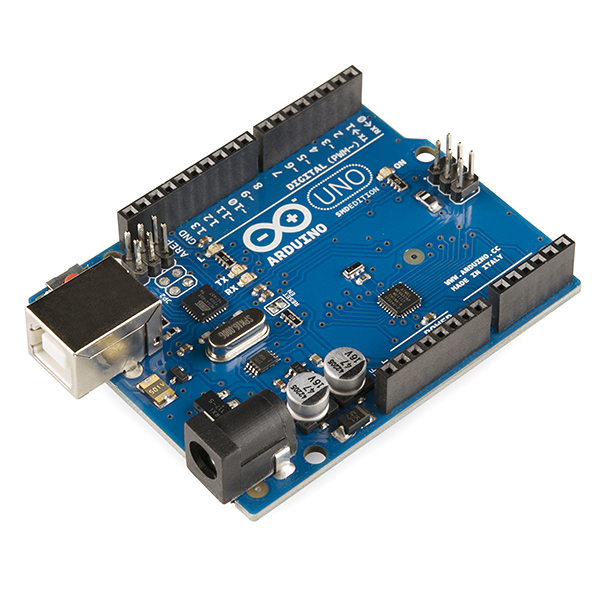
\includegraphics[width=25mm]{pic/arduino.jpg}
    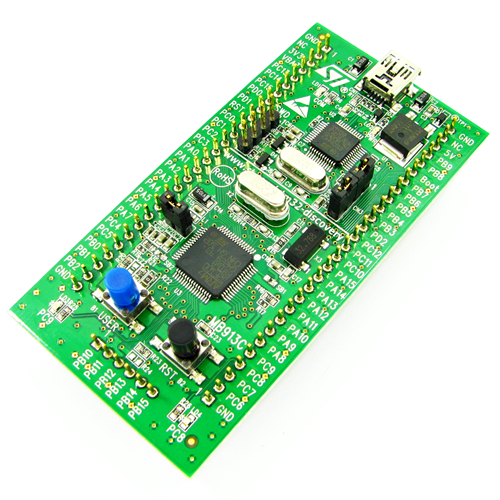
\includegraphics[width=25mm]{pic/stm32.png}
    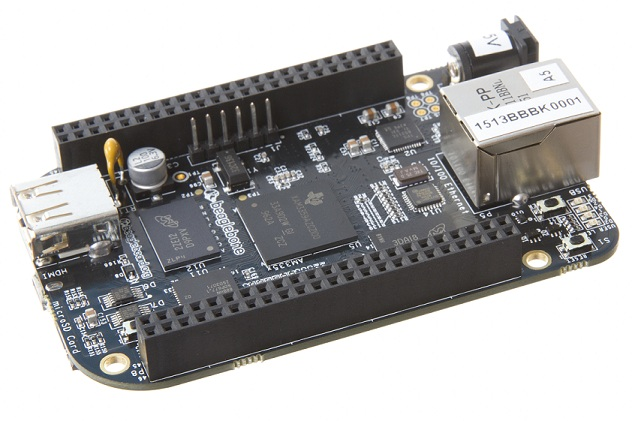
\includegraphics[width=25mm]{pic/bbb.jpg}
    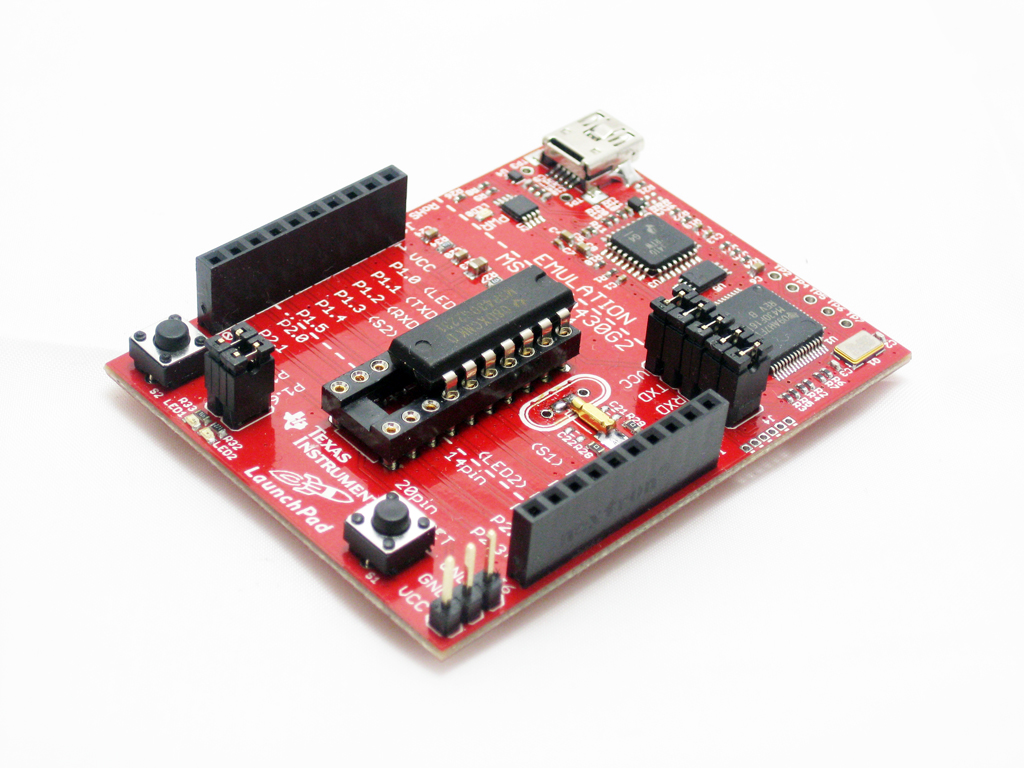
\includegraphics[width=25mm]{pic/msp430.jpg}
  \end{center}

  \begin{small}
    \begin{itemize}
    \item Multiplication des solutions pour l'embarqu\'{e}
    \item Compromis: puissance, p\'{e}riph\'{e}riques, c\^out, complexit\'{e}, support ...
      \begin{itemize}
      \item[\checkmark] La BeagleBone Black s'impose dans sa cat\'egorie
      \end{itemize}
    \end{itemize}
  \end{small}

\end{frame}


\begin{frame}{BBB - Caract\'eristiques mat\'{e}rielles}
  \begin{center}
    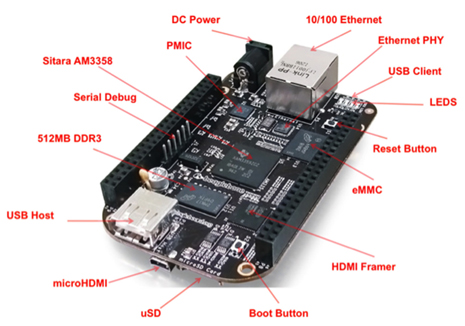
\includegraphics[width=40mm]{./pic/bbb_overview.png}
    \hspace{10.00mm}
    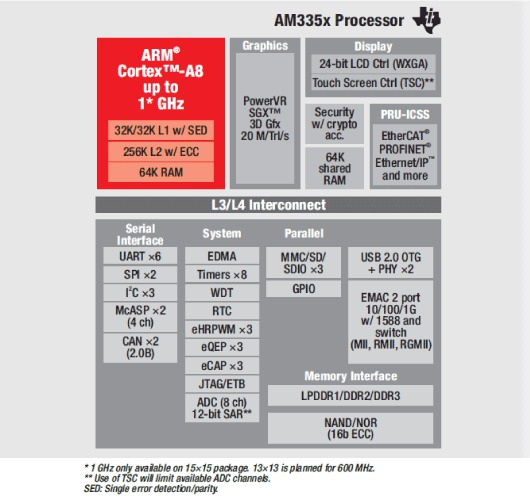
\includegraphics[width=40mm]{./pic/arm335x_dia.jpg}
  \end{center}

  \begin{tiny}
    \begin{itemize}
    \item Processeur: AM335x 1GHz ARM Cortex-A8
    \item M\'emoire RAM: 512MB DDR3
    \item Flash int\'egr\'ee: 4GB eMMC
    \item Connectivit\'e: Ethernet, USB (client et h\^ote)
    \item P\'eriph\'erie: UART, I2C, SPI, CAN, PWM, ADC ...
    \item Extension: 2x 46 pin headers
    \end{itemize}
  \end{tiny}
\end{frame}


\begin{frame}{BBB - Cartes d'extension, les \textit{capes}}
  \begin{center}
    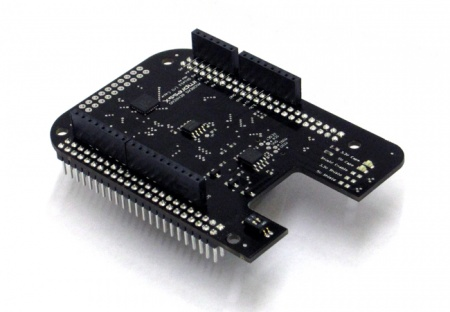
\includegraphics[width=40mm]{./pic/cape_shield.jpg}
    \hspace{4.00mm}
    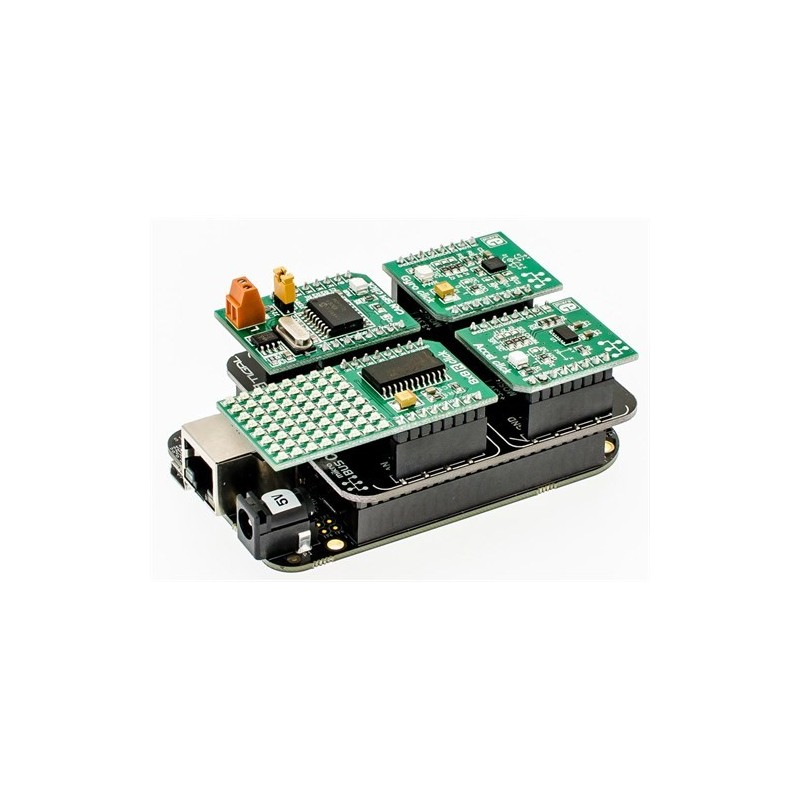
\includegraphics[width=30mm]{./pic/cape_mikrobus.jpg}
  \end{center}

  \begin{tiny}
    \begin{itemize}
    \item Capteurs et acquisition
    \item Logique (FPGA ...)
    \item Affichage (LCD ...)
    \item Communication (CAN, radio ...)
    \item Prototypage
    \item \url{http://elinux.org/Beagleboard:BeagleBone_Capes}
    \end{itemize}
  \end{tiny}

\end{frame}


\begin{frame}{BBB - Support}
  \begin{small}
    \begin{itemize}
    \item Texas Instrument
      \begin{itemize}
      \item processeur ARM3358
      \item \url{http://processors.wiki.ti.com/index.php/Sitara}
      \end{itemize}
    \item Farnell Element14
      \begin{itemize}
      \item Communaut\'{e} (forums ...)
      \item \url{http://www.element14.com/BeagleBone-Black}
      \end{itemize}
    \end{itemize}
  \end{small}
\end{frame}


\begin{frame}{BBB - Exemple d'application: robotique}

  \begin{center}
    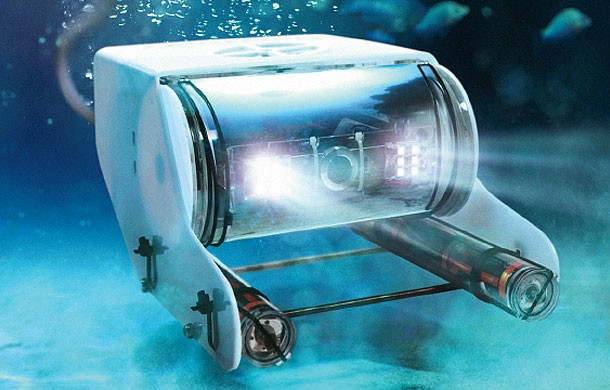
\includegraphics[width=20mm]{./pic/openrov_outside.jpg}
    \hspace{0.500mm}
    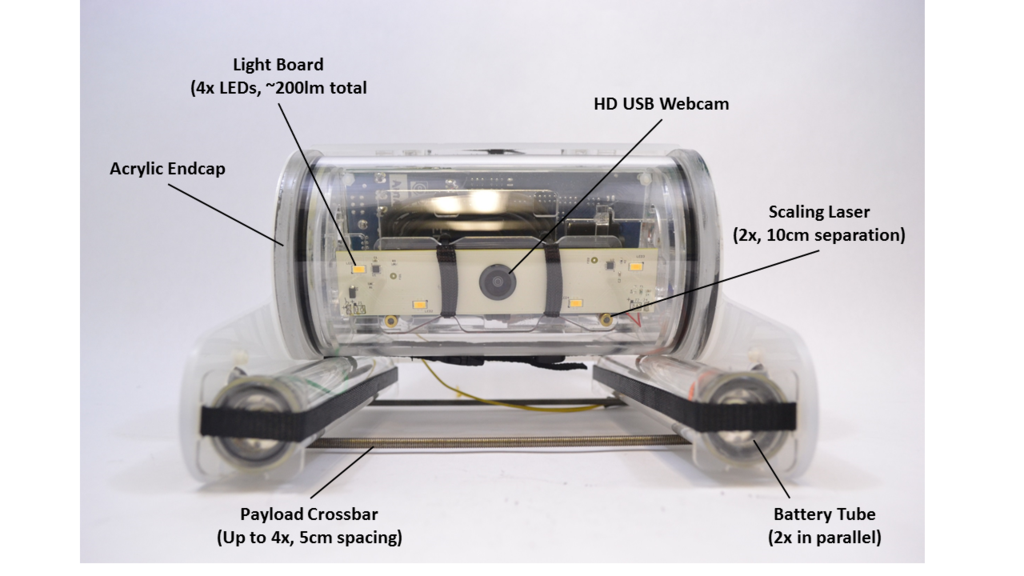
\includegraphics[width=30mm]{./pic/openrov_front.jpg}
    \hspace{0.500mm}
    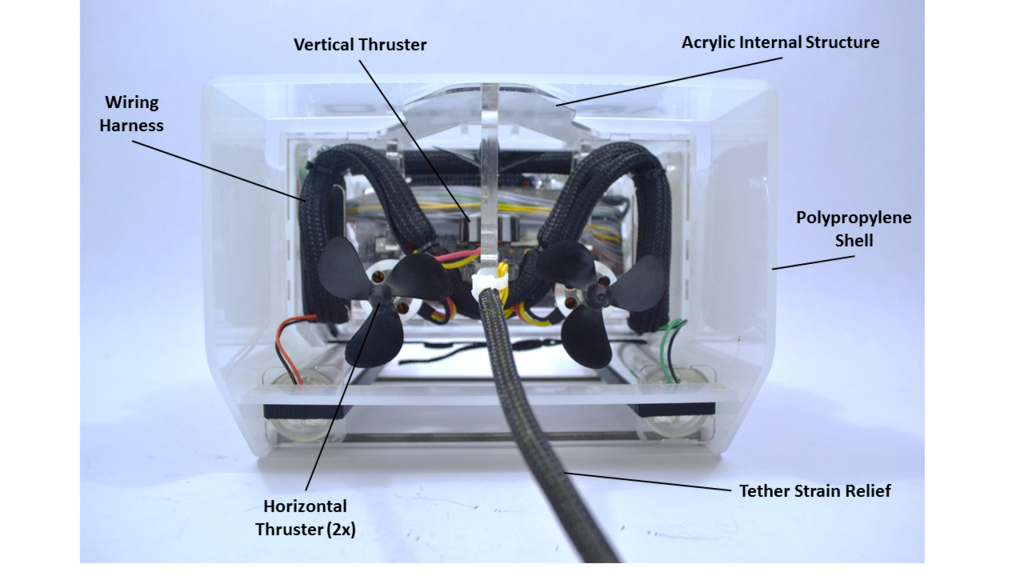
\includegraphics[width=30mm]{./pic/openrov_back.jpg}
    \hspace{0.500mm}
    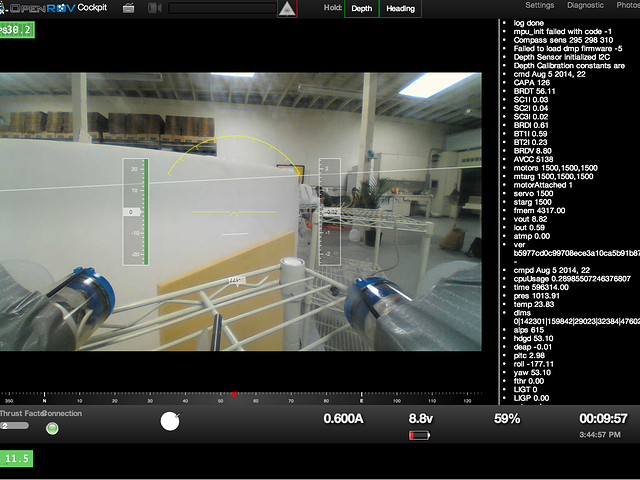
\includegraphics[width=20mm]{./pic/openrov_cockpit.png}
  \end{center}

  \begin{small}
    \begin{itemize}
    \item OpenROV
    \item Webcam, propulsion, \'{e}clairage, serveur http (NodeJS)
    \item \url{http://openrov.com}
    \end{itemize}
  \end{small}

\end{frame}


\begin{frame}{BBB - Exemple d'application: domotique}

  \begin{center}
    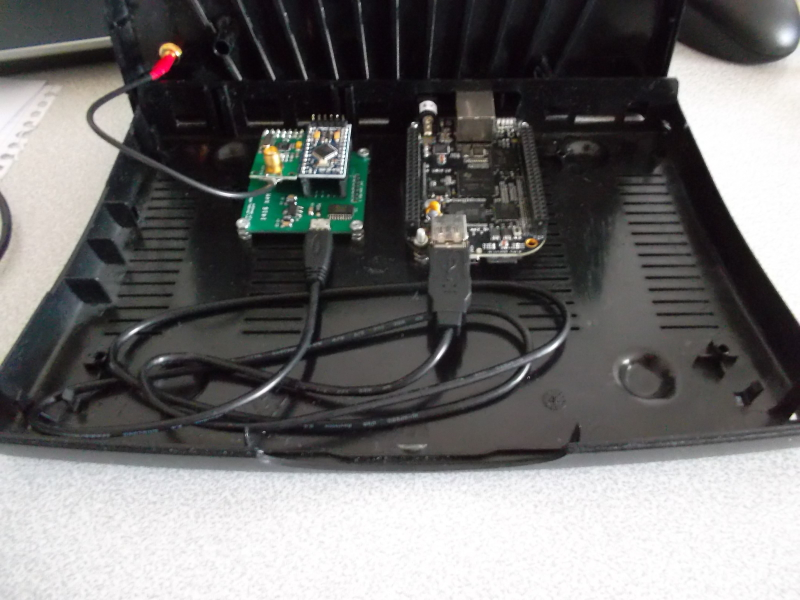
\includegraphics[width=30mm]{./pic/bano_inside.jpg}
    \hspace{2.00mm}
    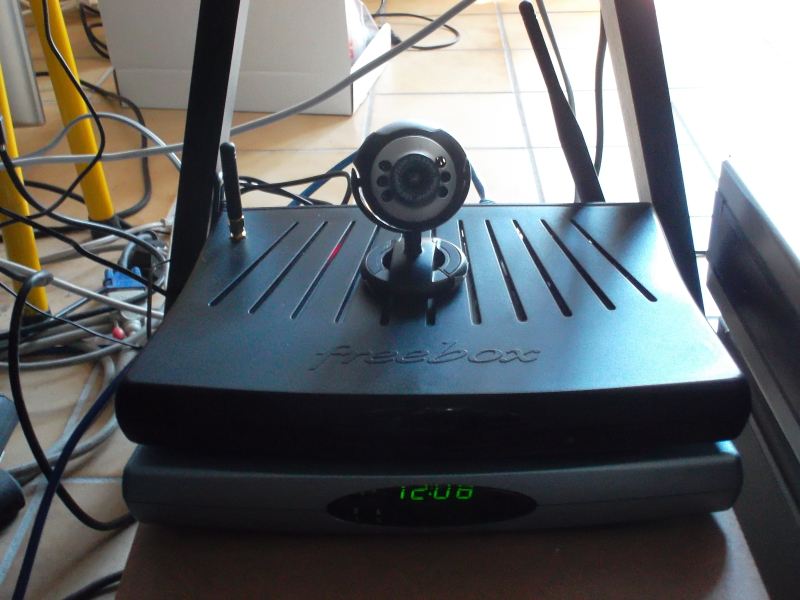
\includegraphics[width=30mm]{./pic/bano_outside.jpg}
    \hspace{2.00mm}
    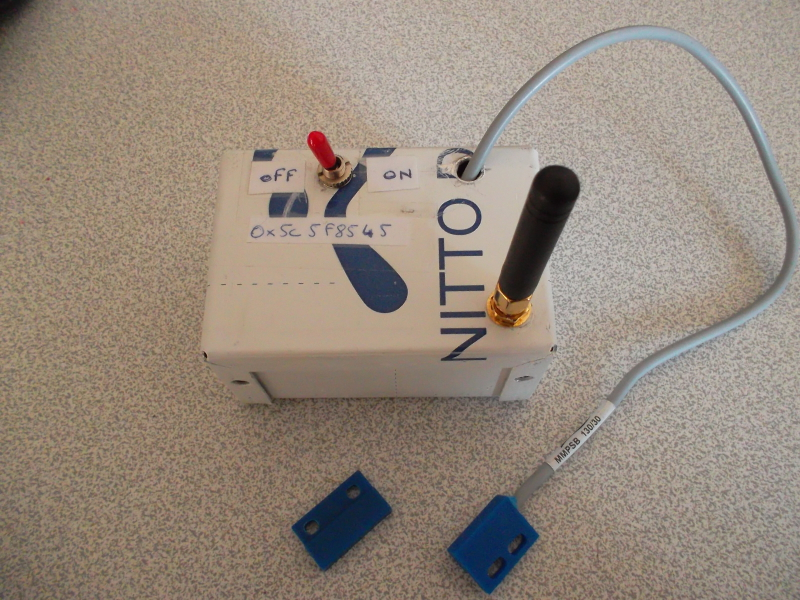
\includegraphics[width=30mm]{pic/bano_reed.jpg}
  \end{center}

  \begin{small}
    \begin{itemize}
    \item BANO
    \item Dongle NRF, webcam, serveur http (Mongoose)
    \item \url{https://github.com/texane/bano}
    \item \url{https://github.com/texane/bano_reed}
    \end{itemize}
  \end{small}

\end{frame}


\begin{frame}{BBB - Exemple d'application: SDR}

  \begin{center}
    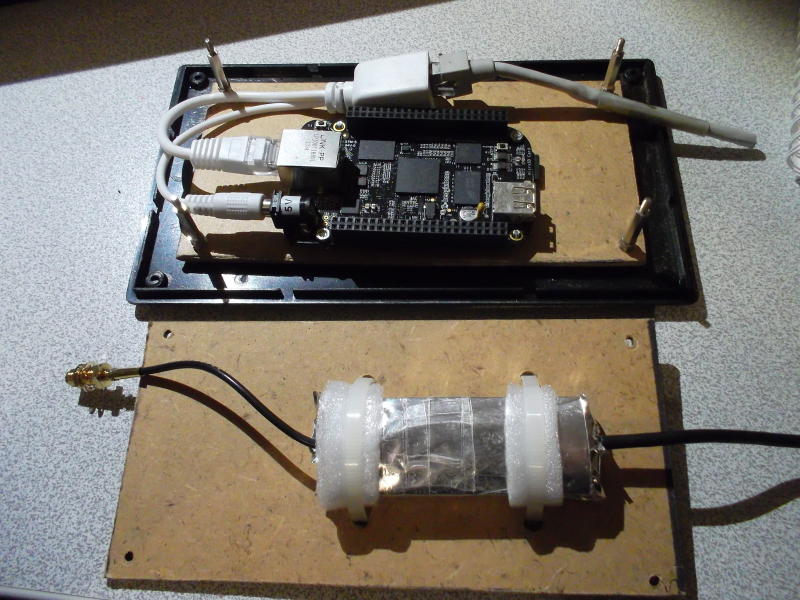
\includegraphics[width=30mm]{./pic/sdrbox_inside.jpg}
    \hspace{2.00mm}
    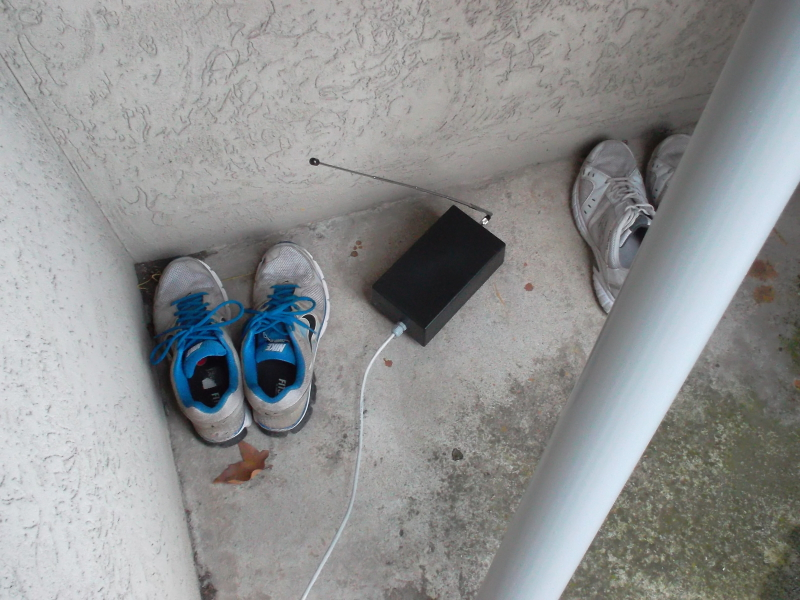
\includegraphics[width=30mm]{./pic/sdrbox_outside.jpg}
  \end{center}

  \begin{small}
    \begin{itemize}
    \item Dongle USB Realtek, librtlsdr
    \end{itemize}
  \end{small}

\end{frame}


\begin{frame}{BBB - R\'{e}f\'{e}rences}
  \begin{small}
    \begin{itemize}
    \item \url{http://beagleboard.org/black}
    \item \url{http://elinux.org/Beagleboard:BeagleBoneBlack}
    \end{itemize}
  \end{small}
\end{frame}


\begin{frame}{Temps r\'eel - D\'efinition}
  Certaines applications n\'ecessitent qu'une partie du code s'\'ex\'ecute
  pr\'ecis\'ement dans le temps. On parle d'applications \textit{temps r\'eel}.
  \newline
  \newline
  L'ordre de grandeur varie selon l'application, et d\'epend largement des
  processus physiques impliqu\'es.
  \newline
  \newline
  Exemples:
  \begin{itemize}
  \item Pilotage de moteurs CNC: microsecondes
  \item Contr\^ole alimentation secteur: millisecondes
  \item Asservissement en temp\'{e}rature: secondes
  \end{itemize}
\end{frame}


\begin{frame}{Temps r\'eel - Probl\'ematique}
  Il est difficile de garantir le respect des contraintes temporelles d\`es
  lors que le code de l'application partage les resources (CPU, memoire, IOs ...)
  avec un autre code plus prioritaire et non pr\'evu pour cela (Linux).
\end{frame}


\begin{frame}{Temps r\'eel - Solutions pour Linux}

  2 types de solutions

  \begin{itemize}
  \item Modification du noyau
    \begin{itemize}
    \item Realtime Linux
    \item Xenomai
    \end{itemize}

  \item Coprocesseurs d\'edi\'es
    \begin{itemize}
    \item Auxiliaires: microcontr\^oleur, FPGA
    \item Int\'egr\'es: \textbf{PRU}, Zynq, coeur d\'edi\'e
    \end{itemize}

  \end{itemize}
\end{frame}


\begin{frame}{PRU - Introduction}

  \begin{center}
    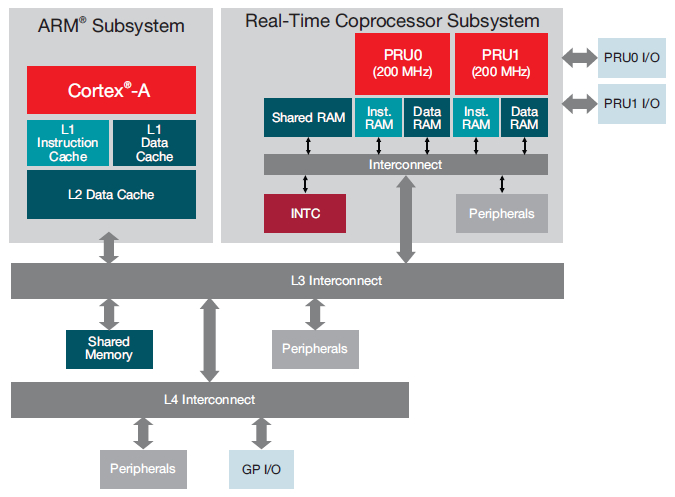
\includegraphics[width=45mm]{./pic/pru_interconnect.jpg}
  \end{center}

  \begin{tiny}
    Le processeur de la BBB int\`egre 2 microcontr\^oleurs d\'edi\'es \`a l'application: les \textbf{PRU}s
    \begin{itemize}
    \item \textbf{P}rogrammable \textbf{R}ealtime \textbf{U}nit
    \item Pas de syst\`eme d'exploitation
    \item 200MHz 32 bits RISC, 5 ns par instruction
    \item M\'emoire locales (instructions: 8KB, donn\'ees: 8KB), partag\'ee (12KB)
    \item P\'eriph\'eriques d\'edi\'es (5ns latency Enhanced GPIOs)
    \item Acc\`es \`a la totalit\'e des p\'eriph\'eriques via un bus d'interconnection
    \item Communication processeur (m\'emoire partag\'ee, interruptions)
    \end{itemize}
  \end{tiny}

\end{frame}


\begin{frame}{PRU - Applications}

  \begin{center}
    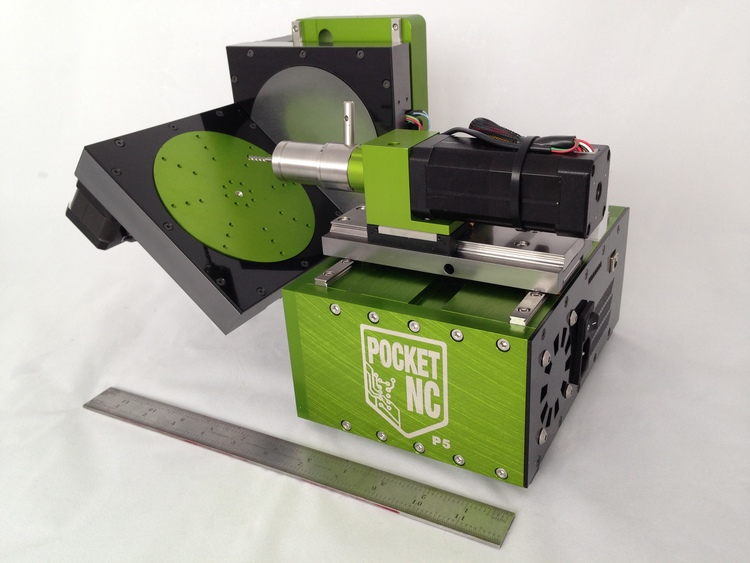
\includegraphics[width=35mm]{pic/pocketnc.jpg}
    \hspace{0.400mm}
    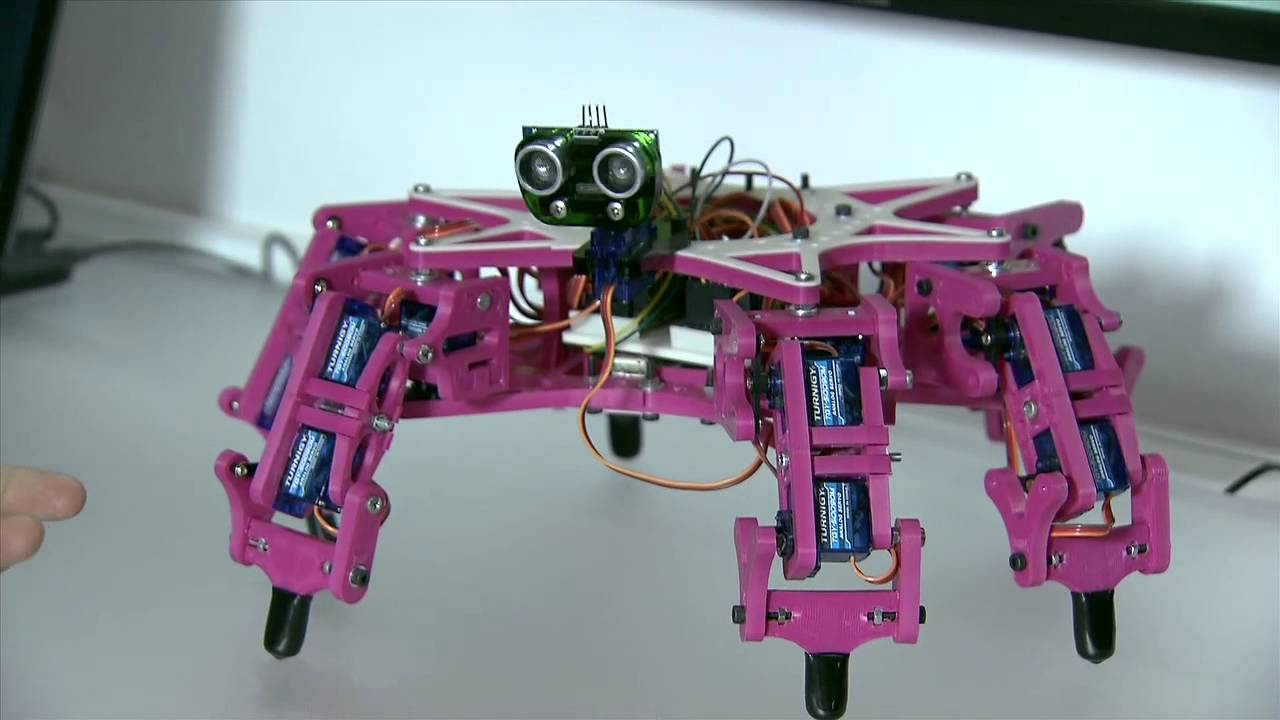
\includegraphics[width=35mm]{pic/spiderbot.jpg}
    \hspace{0.400mm}
    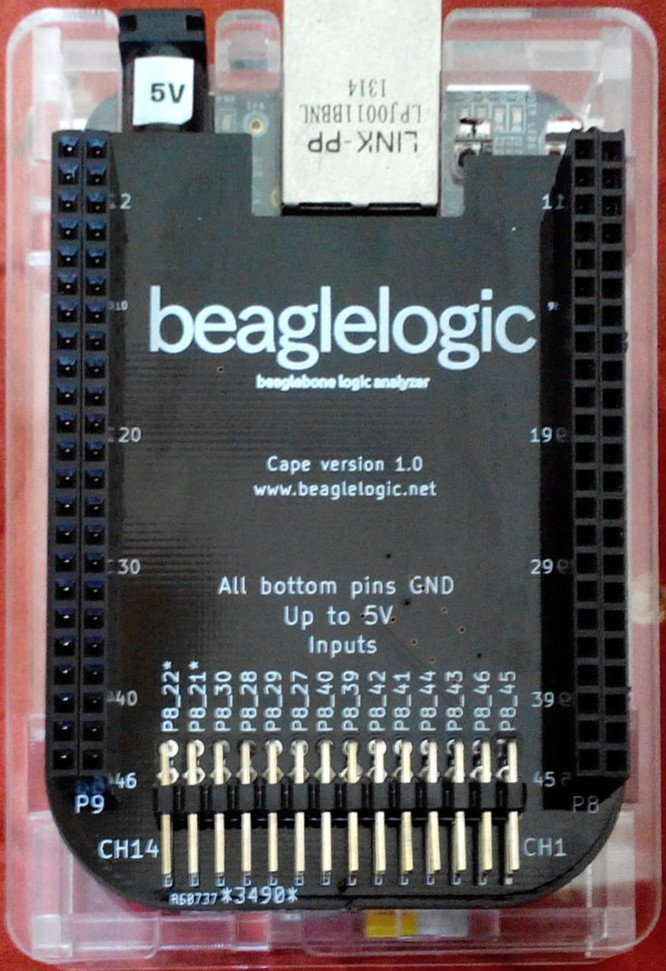
\includegraphics[height=30mm]{pic/beaglelogic.jpg}
  \end{center}

  \begin{small}
    \begin{itemize}
    \item Contr\^ole et asservissement: CNC, robots ...
    \item Mesure et instrumentation
    \item \url{http://processors.wiki.ti.com/index.php/PRU_Projects}
    \end{itemize}
  \end{small}
\end{frame}


\begin{frame}{PRU - Workflow}

  \begin{small}

    Pr\'eparation
    \begin{itemize}
    \item Installation toolchain GNU et PRU
    \item Compilation noyau (activation driver PRUSS)
    \item Cr\'eation d'une image disque
    \end{itemize}

    D\'eveloppement
    \begin{itemize}
    \item Programmes h\^ote et PRU
    \item Script device tree
    \end{itemize}

    Lancement de l'application
    \begin{itemize}
    \item Chargement driver et overlay device tree
    \item Lancement programme h\^ote
    \end{itemize}

  \end{small}

\end{frame}


\begin{frame}{PRU - Installation toolchain GNU pour ARM}
  \begin{small}
    N\'ecessaire pour compiler les programmes h\^otes et le noyau.\\
    Diff\'erentes m\'ethodes:
    \begin{itemize}
    \item crosstool-ng
      \begin{itemize}
      \item \begin{tiny} \url{https://github.com/texane/lfs/blob/master/board/bbb/crosstool-ng-1.18.0.config} \end{tiny}
      \end{itemize}
    \item gestionnaire de paquets
      \begin{itemize}
      \item \begin{tiny} aptitude install gcc-4.7-arm-linux-gnueabi \end{tiny}
      \end{itemize}
    \item \url{http://elinux.org/Building_BBB_Kernel}
    \end{itemize}
  \end{small}
\end{frame}


\begin{frame}{PRU - Installation toolchain PRU}
  \begin{small}
    N\'ecessaire pour compiler les programmes PRU
    \begin{itemize}
    \item \url{http://github.com/texane/pru_sdk}
    \item \url{http://www.embeddedrelated.com/showarticle/586.php}
    \end{itemize}
  \end{small}
\end{frame}


\begin{frame}{PRU - Compilation noyau Linux}
  \begin{small}
    N\'ecessaire pour activer le driver PRU
    \begin{itemize}
    \item version 3.8.13
    \item CONFIG\_UIO\_PRUSS=m
    \item modprobe uio\_pruss
    \item \begin{tiny} \url{https://github.com/texane/lfs/blob/master/board/bbb/linux-3.8.13.config} \end{tiny}
    \end{itemize}
  \end{small}
\end{frame}


\begin{frame}{PRU - Cr\'eation d'une image disque}
  \begin{small}
    Utilisation de l'outil LFS
    \begin{itemize}
    \item \url{https://github.com/texane/lfs}
    \item Compile aussi une toolchain GNU et un noyau
    \item L'image produite se copie via dd sur une carte SD
    \end{itemize}
  \end{small}
\end{frame}


\begin{frame}{PRU - Overlay Device Tree (1)}

  \textit{Device Tree} est un sous syst\`eme de Linux qui
  d\'ecrit le mat\'eriel au noyau sous la forme d'une
  arborescence de p\'eriph\'eriques:
  \begin{itemize}
  \item \begin{tiny} \url{http://elinux.org/Device_Tree} \end{tiny}
  \item \begin{tiny} \url{petazzoni-device-tree-dummies.pdf} \end{tiny}
  \item \begin{tiny} \url{http://hipstercircuits.com/beaglebone-black-gpio-mux-for-pru-with-device-tree-overlay/} \end{tiny} \newline
  \end{itemize}

  Un script Device Tree (xxx.dts) est n\'ecessaire pour modifier,
  \'etendre ou surcharger cette arboresence. On parle aussi
  d'\textit{overlay}. Dans notre cas:
  \begin{itemize}
  \item Activer le PRU
  \item Configurer le multiplexeur des IOs
  \end{itemize}

\end{frame}


\begin{frame}{PRU - Overlay Device Tree (2)}

  L'overlay se compile en un binaire (xxx.dtbo) puis se copie
  sur la cible dans dans un r\'epertoire particulier:
  \begin{itemize}
  \item dtc -@ -O dtb -o xxx.dtbo xxx.dts
  \item cp xxx.dtbo /lib/firmware/ \newline
  \end{itemize}

  Avant l'\'ex\'ecution du programme, l'overlay doit \^etre
  ajout\'e \`a l'arborescence des p\'eriph\'eriques du noyau:
  \begin{itemize}
  \item echo \textit{part\_number} $>$ /sys/devices/bone\_capemgr.9/slots
  \item \textit{part\_number} est un identifiant d\'efini dans
    l'overlay
  \end{itemize}

\end{frame}


\begin{frame}[containsverbatim]{PRU - Overlay Device Tree (3)}
  \begin{tiny} V\'erification du chargement via dmesg \end{tiny}
  \lstset{commentstyle=\color{blue}}
  \lstset{language=C++}
  \lstset{basicstyle=\fontsize{6}{6}\selectfont\ttfamily}
  \begin{lstlisting}[frame=tb]
...
[  996.191234] bone-capemgr bone_capemgr.9: part_number 'gpio_p8_11',
version 'N/A'
[  996.191350] bone-capemgr bone_capemgr.9: slot #8: generic override
[  996.191377] bone-capemgr bone_capemgr.9: bone: Using override eeprom
data at slot 8
[  996.191407] bone-capemgr bone_capemgr.9: slot #8: 'Override Board
Name,00A0,Override Manuf,gpio_p8_11'
[  996.191512] bone-capemgr bone_capemgr.9: slot #8: Requesting part
number/version based 'gpio_p8_11-00A0.dtbo
[  996.191546] bone-capemgr bone_capemgr.9: slot #8: Requesting firmware
'gpio_p8_11-00A0.dtbo' for board-name 'Override Board Name', version '00A0'
[  996.191793] bone-capemgr bone_capemgr.9: slot #8: dtbo 'gpio_p8_11-00A0.dtbo'
loaded; converting to live tree
[  996.192981] bone-capemgr bone_capemgr.9: slot #8: #3 overlays
[  996.195171] bone-capemgr bone_capemgr.9: slot #8: Applied #3 overlays.
  \end{lstlisting}
\end{frame}


\begin{frame}[containsverbatim]{PRU - Overlay Device Tree (4)}
  \begin{tiny} Overlay d'activation du PRU \end{tiny}
  \lstset{commentstyle=\color{blue}}
  \lstset{language=C++}
  \lstset{basicstyle=\fontsize{6}{6}\selectfont\ttfamily}
  \begin{lstlisting}[frame=tb]
/dts-v1/;
/plugin/;

/ {
	compatible = "ti,beaglebone", "ti,beaglebone-black";

	/* identification */
	part-number = "pruss_enable";
	version = "00A0";

 	fragment@0 {
  		   target = <&pruss>;
		   __overlay__ {
		   	       status = "okay";

    	           };
        };

};
  \end{lstlisting}
\end{frame}


\begin{frame}[containsverbatim]{PRU - Overlay Device Tree (5)}
  \begin{tiny}
    Overlay de multiplexage la pin 8.15 en mode PWM
  \end{tiny}
  \lstset{commentstyle=\color{blue}}
  \lstset{language=C++}
  \lstset{basicstyle=\fontsize{6}{6}\selectfont\ttfamily}
  \begin{lstlisting}[frame=tb]
/dts-v1/;
/plugin/;

/ {
	compatible = "ti,beaglebone", "ti,beaglebone-black";

	/* identification */
	part-number = "my_pwm_P8_15";
	version = "00A0";

	fragment@0 {
		target = <&am33xx_pinmux>;
		__overlay__ {
			pwm_P8_15: pinmux_pwm_P8_15_pins {
				pinctrl-single,pins = <0x3c 0x5>;
			};
		};
	};

	fragment@1 {
		target = <&ocp>;
		__overlay__ {
			pwm_test_P8_15 {
				compatible	= "pwm_test";
				pwm-names 	= "PWM_P8_15";
				pinctrl-names	= "default";
				pinctrl-0	= <&pwm_P8_15>;
				enabled		= <1>;
				status 		= "okay";
			};
		};
	};
};
  \end{lstlisting}
\end{frame}


\begin{frame}{PRU - Overlay Device Tree (6)}
  \begin{small}
    En pratique, on copie colle un script existant en changeant les offsets
    et les modes de multiplexage des pins. 2 documentations utiles:
    \begin{itemize}
    \item \begin{tiny} \url{https://github.com/texane/pru_sdk/blob/master/doc/BeagleboneBlackP8HeaderTable.pdf} \end{tiny}
    \item \begin{tiny} \url{https://github.com/texane/pru_sdk/blob/master/doc/BeagleboneBlackP9HeaderTable.pdf} \end{tiny}
    \end{itemize}
  \end{small}
\end{frame}


\begin{frame}{PRU - Programme PRU en assembleur (1)}
  \begin{small}
    Converti un programme \'ecrit dans le langage assembleur
    en un binaire qui sera charg\'e sur le PRU par le programme
    h\^ote:
    \begin{itemize}
    \item pasm -V2 -I\$(PRU\_SDK\_DIR)/include -b xxx.p
    \item Produit xxx.bin
    \end{itemize}
  \end{small}
\end{frame}


\begin{frame}{PRU - Programme PRU en assembleur (2)}
  \begin{small}
    Jeu d'instructions g\'en\'eraliste
    \begin{itemize}
    \item Branchement, arithm\'etique, load store ...
    \item Unit\'e MAC avec saturation
    \item am335xPruReferenceGuide.pdf
    \end{itemize}
  \end{small}
\end{frame}


\begin{frame}[containsverbatim]{PRU - Programme PRU en assembleur (3)}
   \lstset{commentstyle=\color{blue}}
   \lstset{language=C++}
   \lstset{basicstyle=\fontsize{6}{6}\selectfont\ttfamily}
   \begin{lstlisting}[frame=tb]
// blink.pasm

#define GPIO1 0x4804c000
#define GPIO_CLEARDATAOUT 0x190
#define GPIO_SETDATAOUT 0x194

INIT_OCP:
 LBCO r0, C4, 4, 4
 CLR r0, r0, 4
 SBCO r0, C4, 4, 4

 MOV r1, 10

BLINK:
 MOV r2, 7<<22
 MOV r3, GPIO1 | GPIO_SETDATAOUT
 SBBO r2, r3, 0, 4
 MOV r0, 0x00a00000

DELAY:
 SUB r0, r0, 1
 QBNE DELAY, r0, 0
 MOV r2, 7<<22
 MOV r3, GPIO1 | GPIO_CLEARDATAOUT
 SBBO r2, r3, 0, 4
 MOV r0, 0x00a00000

DELAY2:
 SUB r0, r0, 1
 QBNE DELAY2, r0, 0
 SUB r1, r1, 1
 QBNE BLINK, r1, 0
 \end{lstlisting}
\end{frame}


\begin{frame}{PRU - Programme PRU en C (1)}
  \begin{tiny}

    Texas Instrument CSS (celui utilis\'e)
    \begin{itemize}
    \item \url{http://processors.wiki.ti.com/index.php/Download_CCS}
    \item \url{www.embeddedrelated.com/showarticle/603.php}
    \item Celui utilis\'e dans cette conf\'erence \newline
    \end{itemize}

    GNU GCC, portage non officiel
    \begin{itemize}
    \item \url{https://github.com/dinuxbg/gnupru}
    \item difficile \'a installer et fonctionnalit\'es absentes (05/2015)
    \end{itemize}

  \end{tiny}
\end{frame}


\begin{frame}[containsverbatim]{PRU - Programme PRU en C (2)}
 \begin{tiny}
   \lstset{commentstyle=\color{blue}}
   \lstset{language=C++}
   \lstset{basicstyle=\fontsize{6}{6}\selectfont\ttfamily}
   \begin{lstlisting}[frame=tb]
/* blink.c */

#include <pru/io.h>

static void delay_cycles(unsigned int n)
{
  unsigned int i;
  for (i = 0; i < n/2; i++) asm volatile ("nop" : : );
}

static void delay_us(unsigned int us)
{
  /* assume cpu frequency is 200MHz */
  delay_cycles(us * (1000 / 5));
}

const unsigned int period_us = 250 * 1000;

int main(void)
{
  unsigned int c;

  for (c = 0; ; c++)
  {
    write_r30(c & 1 ? 0xffff : 0x0000);
    delay_us(period_us);
  }

  return 0;
}
 \end{lstlisting}
 \end{tiny}
\end{frame}


\begin{frame}[containsverbatim]{PRU - Programme PRU en C (3)}
 \begin{tiny}
   Assembleur inline possible
   \lstset{commentstyle=\color{blue}}
   \lstset{language=C++}
   \lstset{basicstyle=\fontsize{6}{6}\selectfont\ttfamily}
   \begin{lstlisting}[frame=tb]
uint32_t shm_read(register uint32_t i)
{
  /* i is the absolute offset relative from shared memory start */
  /* read x at shm + i */

  __asm__ __volatile__
  (
   " LDI32 r0, 0x000000120 \n"
   " LDI32 r1, 0x22028 \n"
   " SBBO &r0, r1, 0, 4 \n"

   " LDI32 r0, 0x00100000 \n"
   " LDI32 r1, 0x2202c \n"
   " SBBO &r0, r1, 0, 4 \n"

   " LBCO &r14, C31, 0, 4 \n"
   " JMP R3.w2 \n"
  );

  /* unreached */
  return 0;
}
 \end{lstlisting}
 \end{tiny}
\end{frame}


\begin{frame}{PRU - Programme h\^ote (1)}
  \begin{small}
    Le programme h\^ote s'\'ex\'ecute sur le processeur h\^ote.
    Il initialise le PRU et y charge le binaire pr\'ec\'edemment
    compil\'e. En cours d'\'ex\'ecution, l'h\^ote communique avec
    le PRU via de la m\'emoire partag\'ee et des interruptions.
    \begin{itemize}
    \item Communication de consignes
    \item Acquisition de donn\'ees
    \item Attente d'\'ev\'enements
    \end{itemize}
  \end{small}
\end{frame}


\begin{frame}[containsverbatim]{PRU - Programme h\^ote (2)}
 \begin{tiny}
   \lstset{commentstyle=\color{blue}}
   \lstset{language=C++}
   \lstset{basicstyle=\fontsize{4}{4}\selectfont\ttfamily}
   \begin{lstlisting}[frame=tb]
/* main.c */

#include "prussdrv.h"
#include "pruss_intc_mapping.h"

int main(int ac, char** av)
{
  /* initialize the PRU */
  tpruss_intc_initdata pruss_intc_initdata = PRUSS_INTC_INITDATA;
  prussdrv_init();
  if (prussdrv_open(PRU_EVTOUT_0)) return -1;
  prussdrv_pruintc_init(&pruss_intc_initdata);

  /* ... */

  /* execute code on pru0 */
#define PRU_NUM 0
  prussdrv_exec_program(PRU_NUM, "./xxx.bin");

  /* ... */

  /* wait until pru0 finishes */
  prussdrv_pru_wait_event(PRU_EVTOUT_0);
  prussdrv_pru_clear_event(PRU_EVTOUT_0, PRU0_ARM_INTERRUPT);

  /* disable pru and close memory mapping */
  prussdrv_pru_disable(PRU_NUM);
  prussdrv_exit();

  return 0;
}
 \end{lstlisting}
 \end{tiny}
\end{frame}


\begin{frame}{PRU - Environements et outils}
  \begin{tiny}
    Programmation Python
    \begin{itemize}
    \item \url{http://hipstercircuits.com/pypruss-a-simple-pru-python-binding-for-beaglebone}\newline
    \end{itemize}

    D\'eboggage
    \begin{itemize}
    \item \url{http://processors.wiki.ti.com/index.php/PRU_Debugging}
    \item \url{http://sourceforge.net/projects/prudebug}
    \end{itemize}

  \end{tiny}
\end{frame}


\begin{frame}{PRU - R\'ef\'erences}
  \begin{small}
    \begin{itemize}
    \item \url{http://beagleboard.org/pru}
    \item \url{http://elinux.org/Ti_AM33XX_PRUSSv2}
    \item \url{http://processors.wiki.ti.com/index.php/PRU-ICSS}
    \end{itemize}
  \end{small}
\end{frame}


\begin{frame}{D\'emonstration - pru\_sdk/example/pruss\_iep}
  \begin{small}
    Le CPU lit des valeurs \'ecrites par le PRU \`a intervals de
    temps r\'egulier dans une zone de memoire partag\'ee. Le module
    de timers IEP est utilis\'e pour cadencer l'\'ecriture du PRU.
  \end{small}
\end{frame}


\begin{frame}{D\'emonstration - pru\_sdk/example/pruss\_spwm}
  \begin{small}
    Le PRU g\'en\`ere un signal carr\'e. La fr\'equence est donn\'ee
    par le programme h\^ote via une valeur \'ecrite en RAM.
  \end{small}
\end{frame}


\begin{frame}{Questions}
  \begin{center}
    \textbf{Questions ?} \\
    \textbf{Remarques pour un futur atelier ?}
  \end{center}
\end{frame}


\end{document}
